% Based on the template from Pandoc 3.1.2. Custom sections are marked 'CUSTOM'.
% Customisations go in included files where possible, but this isn't always
% possible.
% Options for packages loaded elsewhere
\PassOptionsToPackage{unicode}{hyperref}
\PassOptionsToPackage{hyphens}{url}
\PassOptionsToPackage{dvipsnames,svgnames,x11names}{xcolor}
%
\documentclass[
  12pt,
  a4paper,
]{article}
\usepackage{amsmath,amssymb}
\usepackage{iftex}
\ifPDFTeX
  \usepackage[T1]{fontenc}
  \usepackage[utf8]{inputenc}
  \usepackage{textcomp} % provide euro and other symbols
\else % if luatex or xetex
  \usepackage{unicode-math} % this also loads fontspec
  \defaultfontfeatures{Scale=MatchLowercase}
  \defaultfontfeatures[\rmfamily]{Ligatures=TeX,Scale=1}
\fi
\usepackage{lmodern}
\ifPDFTeX\else
  % xetex/luatex font selection
  \setmainfont[]{TeX Gyre Termes}
\fi
% Use upquote if available, for straight quotes in verbatim environments
\IfFileExists{upquote.sty}{\usepackage{upquote}}{}
\IfFileExists{microtype.sty}{% use microtype if available
  \usepackage[]{microtype}
  \UseMicrotypeSet[protrusion]{basicmath} % disable protrusion for tt fonts
}{}
\usepackage{fancyvrb}
\usepackage{xcolor}
\usepackage[a4paper]{geometry}
\usepackage{color}
\usepackage{fancyvrb}
\newcommand{\VerbBar}{|}
\newcommand{\VERB}{\Verb[commandchars=\\\{\}]}
\DefineVerbatimEnvironment{Highlighting}{Verbatim}{commandchars=\\\{\}}
% Add ',fontsize=\small' for more characters per line
\newenvironment{Shaded}{}{}
\newcommand{\AlertTok}[1]{\textcolor[rgb]{1.00,0.00,0.00}{\textbf{#1}}}
\newcommand{\AnnotationTok}[1]{\textcolor[rgb]{0.38,0.63,0.69}{\textbf{\textit{#1}}}}
\newcommand{\AttributeTok}[1]{\textcolor[rgb]{0.49,0.56,0.16}{#1}}
\newcommand{\BaseNTok}[1]{\textcolor[rgb]{0.25,0.63,0.44}{#1}}
\newcommand{\BuiltInTok}[1]{\textcolor[rgb]{0.00,0.50,0.00}{#1}}
\newcommand{\CharTok}[1]{\textcolor[rgb]{0.25,0.44,0.63}{#1}}
\newcommand{\CommentTok}[1]{\textcolor[rgb]{0.38,0.63,0.69}{\textit{#1}}}
\newcommand{\CommentVarTok}[1]{\textcolor[rgb]{0.38,0.63,0.69}{\textbf{\textit{#1}}}}
\newcommand{\ConstantTok}[1]{\textcolor[rgb]{0.53,0.00,0.00}{#1}}
\newcommand{\ControlFlowTok}[1]{\textcolor[rgb]{0.00,0.44,0.13}{\textbf{#1}}}
\newcommand{\DataTypeTok}[1]{\textcolor[rgb]{0.56,0.13,0.00}{#1}}
\newcommand{\DecValTok}[1]{\textcolor[rgb]{0.25,0.63,0.44}{#1}}
\newcommand{\DocumentationTok}[1]{\textcolor[rgb]{0.73,0.13,0.13}{\textit{#1}}}
\newcommand{\ErrorTok}[1]{\textcolor[rgb]{1.00,0.00,0.00}{\textbf{#1}}}
\newcommand{\ExtensionTok}[1]{#1}
\newcommand{\FloatTok}[1]{\textcolor[rgb]{0.25,0.63,0.44}{#1}}
\newcommand{\FunctionTok}[1]{\textcolor[rgb]{0.02,0.16,0.49}{#1}}
\newcommand{\ImportTok}[1]{\textcolor[rgb]{0.00,0.50,0.00}{\textbf{#1}}}
\newcommand{\InformationTok}[1]{\textcolor[rgb]{0.38,0.63,0.69}{\textbf{\textit{#1}}}}
\newcommand{\KeywordTok}[1]{\textcolor[rgb]{0.00,0.44,0.13}{\textbf{#1}}}
\newcommand{\NormalTok}[1]{#1}
\newcommand{\OperatorTok}[1]{\textcolor[rgb]{0.40,0.40,0.40}{#1}}
\newcommand{\OtherTok}[1]{\textcolor[rgb]{0.00,0.44,0.13}{#1}}
\newcommand{\PreprocessorTok}[1]{\textcolor[rgb]{0.74,0.48,0.00}{#1}}
\newcommand{\RegionMarkerTok}[1]{#1}
\newcommand{\SpecialCharTok}[1]{\textcolor[rgb]{0.25,0.44,0.63}{#1}}
\newcommand{\SpecialStringTok}[1]{\textcolor[rgb]{0.73,0.40,0.53}{#1}}
\newcommand{\StringTok}[1]{\textcolor[rgb]{0.25,0.44,0.63}{#1}}
\newcommand{\VariableTok}[1]{\textcolor[rgb]{0.10,0.09,0.49}{#1}}
\newcommand{\VerbatimStringTok}[1]{\textcolor[rgb]{0.25,0.44,0.63}{#1}}
\newcommand{\WarningTok}[1]{\textcolor[rgb]{0.38,0.63,0.69}{\textbf{\textit{#1}}}}
\usepackage{graphicx}
\makeatletter
\def\maxwidth{\ifdim\Gin@nat@width>\linewidth\linewidth\else\Gin@nat@width\fi}
\def\maxheight{\ifdim\Gin@nat@height>\textheight\textheight\else\Gin@nat@height\fi}
\makeatother
% Scale images if necessary, so that they will not overflow the page
% margins by default, and it is still possible to overwrite the defaults
% using explicit options in \includegraphics[width, height, ...]{}
\setkeys{Gin}{width=\maxwidth,height=\maxheight,keepaspectratio}
% Set default figure placement to htbp
\makeatletter
\def\fps@figure{htbp}
\makeatother
\ifLuaTeX
  \usepackage{luacolor}
  \usepackage[soul]{lua-ul}
\else
  \usepackage{soul}
\fi
\setlength{\emergencystretch}{3em} % prevent overfull lines
\providecommand{\tightlist}{%
  \setlength{\itemsep}{0pt}\setlength{\parskip}{0pt}}
\setcounter{secnumdepth}{-\maxdimen} % remove section numbering
\ifLuaTeX
\usepackage[bidi=basic]{babel}
\else
\usepackage[bidi=default]{babel}
\fi
\babelprovide[main,import]{british}
\ifPDFTeX
\else
\babelfont[british]{rm}[]{TeX Gyre Termes}
\fi
% get rid of language-specific shorthands (see #6817):
\let\LanguageShortHands\languageshorthands
\def\languageshorthands#1{}
\usepackage{bold-extra}
\usepackage[perpage,symbol*]{footmisc}
\usepackage[labelformat=empty]{caption}

\usepackage{titlesec}

\special{pdf:trailerid [
    <e39b4b5abc3ebb895c799e1e6f5711ab>
    <e39b4b5abc3ebb895c799e1e6f5711ab>
]}
\usepackage{titletoc}
\titlecontents{section}[2.4em]{}{}{\hspace*{-2.4em}}{ \titlerule\contentspage}
\usepackage{titletoc}
\titlecontents{section}[2.4em]{}{}{\hspace*{-2.4em}}{ \titlerule\contentspage}
\ifLuaTeX
  \usepackage{selnolig}  % disable illegal ligatures
\fi
\IfFileExists{bookmark.sty}{\usepackage{bookmark}}{\usepackage{hyperref}}
\IfFileExists{xurl.sty}{\usepackage{xurl}}{} % add URL line breaks if available
\urlstyle{same}
\VerbatimFootnotes % allow verbatim text in footnotes
\hypersetup{
  pdftitle={Test 4},
  pdfauthor={The Author},
  pdflang={en-GB},
  pdfsubject={Version: reproducible},
  colorlinks=true,
  linkcolor={black},
  filecolor={Maroon},
  citecolor={Blue},
  urlcolor={Blue},
  pdfcreator={LaTeX via pandoc}}

\title{Test 4}
\author{The Author}
\date{1 January 2022}

\begin{document}
\maketitle

\frenchspacing

\newcommand{\sectionbreak}{\clearpage}

\thispagestyle{empty}

\thispagestyle{empty}

{
\hypersetup{linkcolor=}
\setcounter{tocdepth}{1}
\tableofcontents
}

\hypertarget{__h1_1}{%
\section{The Title}\label{__h1_1}}

\makeatletter
\@afterindentfalse
\@afterheading
\makeatother

This is some text before a section. It shouldn't be indented.

\hypertarget{__h2_1}{%
\subsection{This is a section}\label{__h2_1}}

\makeatletter
\@afterindentfalse
\@afterheading
\makeatother

This is some test text. This is formatted in \emph{italics} and
\textbf{bold}, with - various -- dashes---, and trailing dots\ldots{}

This is a bullet list:

\begin{itemize}
\item
  This is the first paragraph of the first item.

  And the second paragraph of the first item.
\item
  The second item only has one paragraph.
\end{itemize}

\makeatletter
\@afterindentfalse
\@afterheading
\makeatother

This is a numbered list:

\begin{enumerate}
\def\labelenumi{\arabic{enumi}.}
\item
  This is the first paragraph of the first item.

  And the second paragraph of the first item.
\item
  The second item only has one paragraph.
\end{enumerate}

\makeatletter
\@afterindentfalse
\@afterheading
\makeatother

`These quotes should be curly,' and ``so should these.'' There should be
a blank line before the next paragraph:

~

\makeatletter
\@afterindentfalse
\@afterheading
\makeatother

And then there should be some text \textsuperscript{in~superscript} and
\textsubscript{in~subscript}, and a footnote\footnote{This is a
  footnote. It should appear at the bottom of the page.} with a star, a
footnote\footnote{Another footnote.} with a dagger, and this should be
\texttt{monospace}.

\hypertarget{__h3_1}{%
\subsubsection{Subsection}\label{__h3_1}}

\makeatletter
\@afterindentfalse
\@afterheading
\makeatother

Test text test text test text.

\begin{quote}
This is a quote block. It should be indented slightly and shouldn't
contain a line break.

This is a second paragraph in the same quote block.
\end{quote}

\begin{quote}
This is a quoted line block. It should be indented slightly\\
and have a \emph{line break} after `slightly', and \textbf{formatting}.
\end{quote}

\begin{quote}
``These literal double curly quotes, used where smart\\
quotes gets it wrong, curl the right way even though\\
they're on different lines.''
\end{quote}

\begin{quote}
`These literal single curly quotes, used where smart\\
quotes gets it wrong, curl the right way even though\\
they're on different lines.'
\end{quote}

\makeatletter
\@afterindentfalse
\@afterheading
\makeatother

After this line there should be stars.

\begin{center}* * *\end{center}

\makeatletter
\@afterindentfalse
\@afterheading
\makeatother

This is a new paragraph after the stars. This text is \textsc{Small
Caps}. Here is a pound sign (£), a euro sign (€), and three letters with
accents: ëóû.

\hypertarget{__h1_2}{%
\section{The Title}\label{__h1_2}}

\makeatletter
\@afterindentfalse
\@afterheading
\makeatother

\textbf{An Author}

~

\makeatletter
\@afterindentfalse
\@afterheading
\makeatother

This is some text before a section. It shouldn't be indented. Each
section should start on a new page (but subsections shouldn't).

\hypertarget{__h2_2}{%
\subsection{This is a section}\label{__h2_2}}

\makeatletter
\@afterindentfalse
\@afterheading
\makeatother

This is some test text. This is formatted in \emph{italics} and
\textbf{bold}, with - various -- dashes---, and trailing dots\ldots{}

`These quotes should be curly,' and ``so should these.'' There should be
a blank line before the next paragraph:

~

\makeatletter
\@afterindentfalse
\@afterheading
\makeatother

And then there should be some text \textsuperscript{in~superscript} and
\textsubscript{in~subscript}, and a footnote\footnote{This is a
  footnote. It should appear at the bottom of the page.} with a star, a
footnote\footnote{Another footnote.} with a dagger, and this should be
\texttt{monospace}.

\hypertarget{__h3_2}{%
\subsubsection{Subsection}\label{__h3_2}}

\makeatletter
\@afterindentfalse
\@afterheading
\makeatother

Test text test text test text.

\begin{quote}
This is a quote block. It should be indented slightly and shouldn't
contain a line break.
\end{quote}

\begin{quote}
This is a quoted line block. It should be indented slightly\\
and have a \emph{line break} after `slightly', and \textbf{formatting}.
\end{quote}

\begin{quote}
``These literal double curly quotes, used where smart\\
quotes gets it wrong, curl the right way even though\\
they're on different lines.''
\end{quote}

\begin{quote}
`These literal single curly quotes, used where smart\\
quotes gets it wrong, curl the right way even though\\
they're on different lines.'
\end{quote}

\makeatletter
\@afterindentfalse
\@afterheading
\makeatother

After this line there should be stars.

\begin{center}* * *\end{center}

\makeatletter
\@afterindentfalse
\@afterheading
\makeatother

This is a new paragraph after the stars. This text is \textsc{Small
Caps}. Here is a pound sign (£), a euro sign (€), and three letters with
accents: ëóû.

\hypertarget{__h2_3}{%
\subsection{This is a second section}\label{__h2_3}}

\begin{figure}
\centering
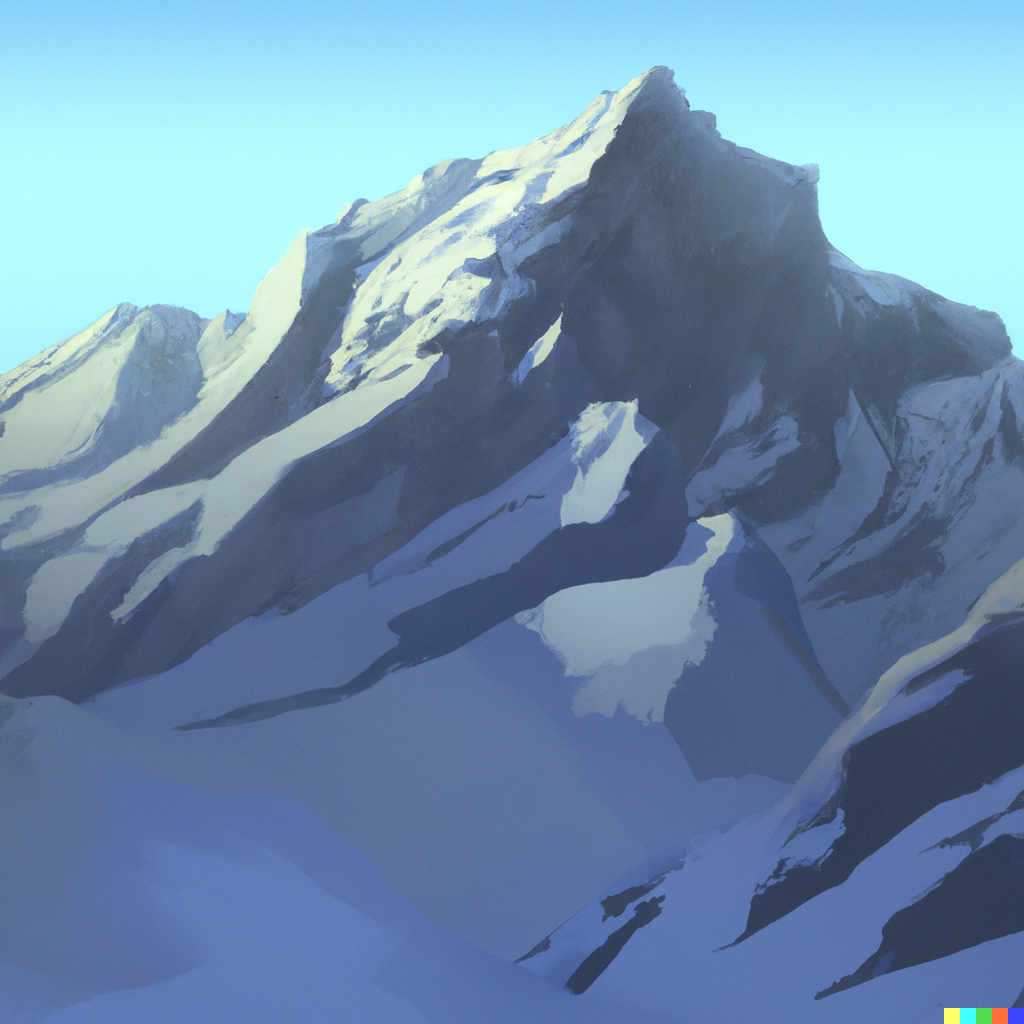
\includegraphics[width=0.5\textwidth,height=\textheight]{tests/test2/image.png}
\caption{foo}
\end{figure}

\makeatletter
\@afterindentfalse
\@afterheading
\makeatother

There is an image here.

And this is \emph{even more italic text}.

\hypertarget{__h1_3}{%
\section{The Title Is `Baz'}\label{__h1_3}}

\makeatletter
\@afterindentfalse
\@afterheading
\makeatother

\textbf{An Author, 23 February 2019 baz}

\hypertarget{__h2_4}{%
\subsection{This is a section}\label{__h2_4}}

\makeatletter
\@afterindentfalse
\@afterheading
\makeatother

This is some test text. This is formatted in \emph{italics} and
\textbf{bold}, with - various -- dashes---, and trailing dots\ldots{}

`These quotes should be curly,' and ``so should these.'' There should be
a blank line before the next paragraph:

~

\makeatletter
\@afterindentfalse
\@afterheading
\makeatother

And then we do a simple include:

Text before a section in simple include.

\hypertarget{__h2_5}{%
\subsection{Section in simple include}\label{__h2_5}}

\begin{quote}
This is a quote block. It should be indented slightly and shouldn't
contain a line break.
\end{quote}

\begin{quote}
This is a quoted line block. It should be indented slightly\\
and have a \emph{line break} after `slightly', and \textbf{formatting}.
\end{quote}

\makeatletter
\@afterindentfalse
\@afterheading
\makeatother

Text before recursive include, with \emph{italic}, \textbf{bold},
``curly quotes,'' and--- an em dash.

Text before section in recursive include.

\hypertarget{__h2_6}{%
\subsection{Section in recursive include}\label{__h2_6}}

\makeatletter
\@afterindentfalse
\@afterheading
\makeatother

Text in recursive include, with \emph{italic}, \textbf{bold}, ``curly
quotes,'' and--- an em dash.

\hypertarget{__h3_3}{%
\subsubsection{Subsection in recursive include}\label{__h3_3}}

\begin{quote}
``These literal double curly quotes, used where smart\\
quotes gets it wrong, curl the right way even though\\
they're on different lines.''
\end{quote}

\begin{quote}
`These literal single curly quotes, used where smart\\
quotes gets it wrong, curl the right way even though\\
they're on different lines.'
\end{quote}

\makeatletter
\@afterindentfalse
\@afterheading
\makeatother

Test text test text test text. After this line there should be stars.

\begin{center}* * *\end{center}

\makeatletter
\@afterindentfalse
\@afterheading
\makeatother

And then there should be some text \textsuperscript{in~superscript} and
\textsubscript{in~subscript}, and a footnote\footnote{This is a
  footnote. It should appear at the bottom of the page.} with a star, a
footnote\footnote{Another footnote.} with a dagger, and this should be
\texttt{monospace}.

Text after recursive include. Here is a pound sign (£), a euro sign (€),
and three letters with accents: ëóû.

\hypertarget{__h2_7}{%
\subsection{Second section in simple include}\label{__h2_7}}

\makeatletter
\@afterindentfalse
\@afterheading
\makeatother

Test text.

Text after simple include.

\hypertarget{__h3_4}{%
\subsubsection{Subsection}\label{__h3_4}}

\makeatletter
\@afterindentfalse
\@afterheading
\makeatother

This is a new paragraph. This text is \textsc{Small Caps}.

\hypertarget{quux-not-spellchecked}{%
\subsection{This is a second section}\label{quux-not-spellchecked}}

\makeatletter
\@afterindentfalse
\@afterheading
\makeatother

And this is \emph{even more italic text}. Foo.

\begin{Shaded}
\begin{Highlighting}[]
\CommentTok{\# Code blocks aren\textquotesingle{}t spellchecked: quux}
\end{Highlighting}
\end{Shaded}

\makeatletter
\@afterindentfalse
\@afterheading
\makeatother

Inline code isn't spellchecked: \texttt{quux}.

\texttt{div} classes aren't spellchecked.

Anything in a nospellcheck div isn't spellchecked: quux.

Automatic links aren't spellchecked: \url{http://quux.com}. Neither are
the targets or attributes of inline links: \href{http://quux.com}{Foo}.
Neither are {span classes}. Anything in a nospellcheck span isn't
spellchecked.

\hypertarget{__h1_4}{%
\section{Title}\label{__h1_4}}

\makeatletter
\@afterindentfalse
\@afterheading
\makeatother

\textbf{4 January 2022}

~

\makeatletter
\@afterindentfalse
\@afterheading
\makeatother

This is text before a section. It shouldn't be indented.

\end{document}
